\documentclass[a4paper]{jarticle}
\setlength{\textwidth}{170mm}
\setlength{\textheight}{260mm}
\setlength{\oddsidemargin}{-5mm}
\setlength{\topmargin}{-25mm}
\usepackage[dvipdfmx]{graphicx}
\usepackage{here}
\usepackage{theorem}
\usepackage{amsmath}
\usepackage{amsfonts}
\usepackage{ascmac}
\usepackage{bm}
\usepackage{comment}
\usepackage{listings,jlisting}
\usepackage{url}

\newtheorem{theo}{定理}[section]
\newtheorem{defi}{定義}[section]
\newtheorem{lemm}{命題}[section]

\title{ベイジアンネットワークによる予測モデルの構築}   %タイトル
\author{小坪琢人}   %著者
\date{\today}   %日付

\makeatletter
\def\theequation{\thesection.\arabic{equation}}   %数式番号を(章.式)形式
\@addtoreset{equation}{section}
\def\thefigure{\thesection.\arabic{figure}}   %図番号を(章.図)形式
\@addtoreset{figure}{section}
\def\thetable{\thesection.\arabic{table}}   %表番号を(章.表)形式
\@addtoreset{table}{section}
\def\tr{\mathop{\operator@font tr}\nolimits}
\def\grad{\mathop{\operator@font grad}\nolimits}
\def\St{\mathop{\operator@font St}\nolimits}
\def\Hess{\mathop{\operator@font Hess}\nolimits}
\def\D{\mathop{\operator@font D}\nolimits}
\def\sym{\mathop{\operator@font sym}\nolimits}
\makeatother

\setlength\textheight{230mm}   %テキスト高さ
\setlength\textwidth{160mm}   %テキスト幅
\setlength{\oddsidemargin}{0mm}   %余白

\begin{document}
\maketitle   %タイトルを付ける
\setlength{\baselineskip}{20pt}   %行間幅
\pagenumbering{roman}   %目次ページ番号のスタイル
\tableofcontents   %目次を付ける
\listoffigures   %図目次を付ける
\listoftables   %表目次を付ける
\clearpage   %目次と本文を分ける
\pagenumbering{arabic}   %本文ページ番号のスタイル

%%%%%これ以下, 本文%%%%%

\section{はじめに}
%%% 2-3ページ  %%%%

現在, 様々な分野で機械学習やディープラーニングが用いられている. その中で自動化というものが大きなテーマであり, 「今後自動化される仕事」のようなニュースも増えている. しかし, マシンの進化により失われる仕事があるのなら, 生まれる新しい仕事も当然存在する. これから生まれる仕事, 必要になる仕事を考えるためには, まず機械学習やディープラーニングでどのようなことができるのかを知る必要がある. 

自動化の問題点としては, 分析やシュミレーションの実態が見えにくくなるという点である. 機械がある種のブラックボックスとなり, 都合よく利用されてしまう可能性がある. 人間が生活していくうえで, 重要視されるのは効率性よりも人間らしい判断である. その中で機械による効率的な自動化は, 意思決定に不信感をもたらす危険性を持っている.

それらを解決する方法として, 可視化というものが存在する. グラフやプロットにより数値的根拠を明らかにすることで, ブラックボックス化を防ぐことができる. 一般に可視化は得られた結果の解釈の手助けとして用いられているが, モデル自体が視覚的に解釈できるものも存在する. 例としては決定木やグラフィカルモデルなどである. 本論文ではこのグラフィカルモデルについて取り上げる. 

%%% グラフィカルモデルの本読んでもう少し書くよ
%%% 因果関係のことどこにいれる??

グラフィカルモデルは以下のような特徴を持つ.~\cite{Bishop1}~\cite{Bishop2}

\begin{enumerate}

\item 確率モデルの構造を視覚化する簡単な方法を提供し, 新しいモデルの設計方針を決めるのに役立つ.

\item グラフの構造を調べることにより, 条件付独立性などのモデルの性質に関する知見が得られる.

\item 精巧なモデルにおいて推論や学習を実行するためには複雑な計算が必要となるが, これを数学的な表現で暗に伴うグラフ上の操作として表現することができる.

\end{enumerate}

グラフはリンク(link)によって接続されたノード(node)の集合からなる. 確率的グラフィカルモデルでは, 各ノードが確率変数を, リンクがこれらの変数間の確率的関係を表現する. 本論では有向グラフィカルとも呼ばれる, ベイジアンネットワーク(Bayesian network)を用いた分類モデルについて議論する.

\section{理論}

\subsection{ベイジアンネットワーク}

ベイジアンネットワークは, 確率変数間の条件付依存関係を表した非循環型有向グラフ(DAG: Directed Acyclic Graph)で, 各種推論などに用いられる. 各ノードは確率変数を表し, 有向辺は変数間の直接の依存関係を表す. 一般には各変数は離散値を取るが, 閾値を定めて離散値に変換すれば連続値にも適用可能である. ベイジアンネットワークでは, リンクの先にあるノードを子ノード$(X_j)$, リンクの元にあるノードを親ノード$(X_i)$と呼ぶ. 親ノードが複数あるとき子ノード$X_j$の親ノードの集合を$Pa(X_j)$と書くことにする. $X_j$と$Pa(X_j)$の間の依存関係は次の条件付確率によって表される. ただし$Pa(X_j)$が空集合の時, $X_j$はベイジアンネットワークの始点であるので, 事前確率分布($P(X_j))$となる.

\begin{eqnarray}
\label{eq1}
P(X_j | Pa(X_j)) = \frac{P(X_j, Pa(X_j))}{P(Pa(X_j))} 
\end{eqnarray}

さらに$n$個の確率変数$X_1, \dots, X_n$のそれぞれを子ノードとして同様に考えると, 全ての確率変数の同時確率分布は式(\ref{eq2})のように表せる.

\begin{eqnarray}
\label{eq2}
P(X_1, \dots, X_n) = \prod_{j=1}^n P(X_j | Pa(X_j))
\end{eqnarray}

上記の式(\ref{eq1})に基づいて, 各ノードについて条件付確率を求めた表を条件付確率表(CPT)といい, 各行の和は必ず$1$になる. 任意の子ノードはそのノードの親ノードのいずれかに起因するので総和は$1$となる (親ノード集合に含まれていないノードを条件とした条件付確率は$0$となる). 条件付確率表の例を表(\ref{cpt})に示す. 

\begin{table}[H]
\begin{center}
\caption{条件付確率表(CPT)}   %キャプション
\label{cpt}   %ラベル
\begin{tabular}{|c||c|c|c|}   %{}で文字の揃え方を指定
\hline
 & $Pa(X_{j})=x_{1}$ & \dots & $Pa(X_{j})=x_{m}$
\\ \hline
$X_j=y_1$ & $p(y_1|Pa(X_j)=x_1)$ & \dots & $p(y_1|Pa(X_j)=x_m)$
\\ \hline
$\vdots$ & $\vdots$ & $\ddots$ & $\vdots$
\\ \hline
$X_j=y_n$ & $ p(y_n|Pa(X_j)=x_1)$ & \dots & $p(y_n|Pa(X_j)=x_m)$
\\ \hline
\end{tabular}
\end{center}
\end{table}

ベイジアンネットワークモデルでは親ノードに対応する変数の値が与えられたとき, 逐次的に各ノードの値も計算される. つまり親ノード以外のノードの値が与えられているとき, ベイズの定理を用いて, 尤もらしい親ノードの値を予測することができる. ベイジアンネットワークによる予測モデルとして, Naive Bayes と Tree Augmented Naive Bayes について説明する.

\subsubsection{Naive Bayes}

Naive Bayes 型のベイジアンネットワークは, 親ノード以外のノードがすべて葉であるような木構造である. ナイーブベイズモデルにおける重要な仮定は, 親ノード以外のノードは, 親ノードに対応する変数の値が与えられた条件の下で条件付独立であるということである. ナイーブベイズモデルの例を図(\ref{naive})に示す.

\begin{figure}[H]
 \begin{center}
  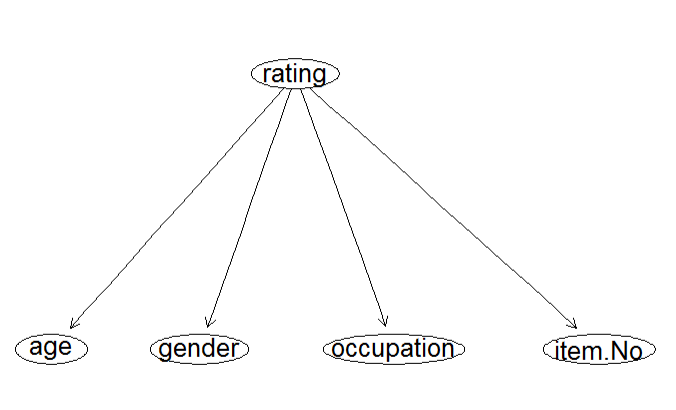
\includegraphics[width=80mm]{data/sample1.png}
 \end{center}
 \caption{ナイーブベイズの例}
 \label{naive}
\end{figure}

構造は常に同様なので, パラメータ学習のみ行う. 訓練データから親ノードと各ノードの値を用いて条件付き確率を求める. 予測を行う際には, 各変数に値を与えてそれぞれ親ノードの値の確率を求め, それらの確率の総和で親ノードの値を決定する.

\subsubsection{Tree Augmented Naive Bayes (TAN)}

TANは, 親ノード以外のノード間が条件付独立であるという Naive Bayes の制約を少し緩めたもので, 子ノード間にも以下に示す条件の下でリンクを与えることができる.~\cite{Friedman}

\begin{itemize}
\item 木構造であること

\item 全ての点の入次数は1以下であること

\item $n$個の説明変数に対して、$n-1$本の有向辺が存在すること
\end{itemize}

TAN 型のベイジアンネットワークを用いた分類器は, 各変数間の依存関係をある程度反映できるため, グラフ構造から視覚的に情報が得られる. TANモデル の例を図(\ref{TAN})に示す.

\begin{figure}[H]
 \begin{center}
  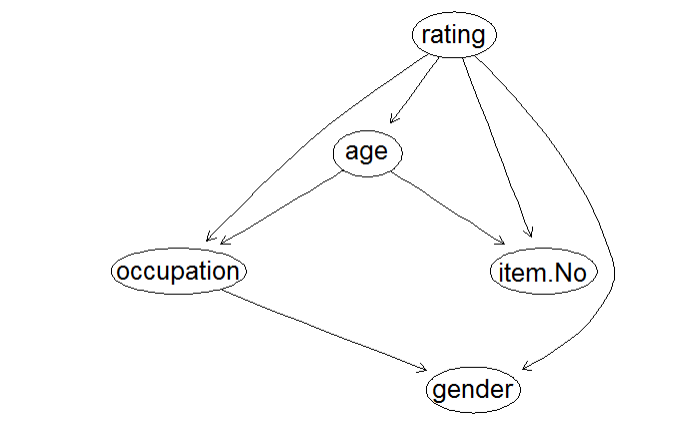
\includegraphics[width=80mm]{data/sample2.png}
 \end{center}
 \caption{Tree Augmented Naive Bayes}
 \label{TAN}
\end{figure}


TAN 型のベイジアンネットワークは Naive Bayes 型のベイジアンネットワークを元に, 関係性の強い説明変数について相互情報量をもとにリンクを与える. その際, 元のクラスラベルの値を条件とした条件付相互情報量を用いる. ここでは条件付相互情報量をTAN 構造の仮定の下で最大化する.

まず, エントロピーについて説明する. エントロピーは式(\ref{entropy})のように表され, 不確かさ(乱雑さ)の指標とされる. $p(x)$は各変数の取りうる値の出現確率を表している. 全ての確率が等しいとき($1/N)$, エントロピーは最大となり, $\log N$となる. あるひとつの値の確率が$1$となり, 他の全ての確率が$0$となるとき, エントロピーは最小となり, $0$である. 同様に結合エントロピー(式(\ref{jointentropy})), 条件付エントロピー, (式(\ref{conditionalentropy}))についても示しておく.

\begin{eqnarray}
\label{entropy}
H(X) &=& - \int_x p(x) \log p(x) 
\end{eqnarray}

\begin{eqnarray}
\label{jointentropy}
H(X, Y) &=& - \int_x \int_y p(x) p(y) \log p(x) \log p(y) \\
\label{conditionalentropy}
H(X| Y) &=& - \int_x \int_y p(x, y) \log p(x| y) dx dy \nonumber \\
           &=& - \int_x \int_y p(x, y) \log p(x, y) dx dy + \int_x \int_y p(x, y) \log p(x) dx dy \nonumber \\
           &=& H(X, Y) - H(Y)
\end{eqnarray}


次に KL情報量(相対エントロピー)~\cite{Meyer}について説明する. KL情報量は式(\ref{KL}) に示したように, 確率分布の近似に用いられる. KL情報量が小さいほど二つの分布が近似していることを表し, $p(x) = q(x)$ となるときKL情報量は$0$となる.

\begin{eqnarray}
\label{KL}
KL(p(x) | q(x)) &=& - \int p(x) \log q(x) dx - \left(- \int p(x) \log p(x) dx \right) \nonumber \\ 
                    &=& - \int p(x) \log \frac{q(x)}{p(x)} dx
\end{eqnarray}

相互情報量と条件付相互情報量について以下のように定義する.

\begin{eqnarray*}
\mbox{相互情報量} &=& I(X, Y) \\
\mbox{条件付相互情報量} &=& I(X, Y | C)
\end{eqnarray*}

ここで相互情報量と条件付相互情報量をKL情報量の式で表すと以下のように表せる. 相互情報量は$X$と$Y$の依存度を表している. 式(\ref{MI})より $X$と$Y$が独立のとき$p(x, y) = p(x) p(y)$となり, KL情報量の定義より $I(X, Y) = 0$となる. すなわち依存関係がある場合に相互情報量は大きくなる. 条件付相互情報量についても同様である. 

\begin{eqnarray}
\label{MI}
I(X, Y) &=& KL(p(x, y) | p(x) q(x)) \nonumber \\
          &=& - \int \int p(x, y) \log \frac{p(x, y)}{p(x) q(x)} dx dy 
\end{eqnarray}

\begin{eqnarray}
\label{CMI}
I(X, Y | Z) &=&  KL(p(x, y| z) | p(x|z) q(x|z)) \nonumber \\
              &=& - \int \int \int p(x, y, z) \log \frac{p(x, y|z)}{p(x|z) q(x|z)} dx dy dz \nonumber \\
               &=& - \int \int \int p(x, y, z) \log p(x, y, z) dx dy dz  \nonumber \\
                &&+ \int \int \int p(x, y, z) \log p(x| z) dx dy dz 
\end{eqnarray}

相互情報量と条件付相互情報量は, エントロピーの定義式(式(\ref{entropy}), 式(\ref{jointentropy}), 式(\ref{conditionalentropy}))を用いて置き換えることができる.  

\begin{eqnarray}
\label{MIentropy}
I(X, Y) &=& H(X) - H(X|Y) \nonumber \\
         &=& H(X) - H(X, Y) + H(Y)
\end{eqnarray}

\begin{eqnarray}
\label{CMIentropy}
I(X, Y | Z) &=& H(X| Z) - H(X| Y, Z) \nonumber \\
               &=& H(X, Z) + H(Y, Z) - H(X, Y, Z) - H(Z)
\end{eqnarray}

TAN 型のベイジアンネットワークでは式(\ref{CMIentropy})に示した, 条件付相互情報量の式を元に親ノード以外のノード間にリンクを与えている. パラメータ学習はナイーブベイズモデルと同様に,  訓練データから親ノードと各ノードの値を用いて条件付き確率を求める. 予測を行う際には, 各変数に値を与えてそれぞれ親ノードの値の確率を求め, それらの確率の総和で親ノードの値を決定する.

\subsection{MDL基準}

MDL(Minimal Description Length)基準は, 離散化手法であるが, 離散値についても分割が適応することができる. (現在調査中)

\section{関連手法}

\subsection{Matrix Factorization}

この手法は協調フィルタリングにおいて次元削減を実現手法である. 協調フィルタリングとはユーザーのレビューをもとに, 同様の評価パターンを持つユーザー同士のデータをもとにまだ評価していない(本質的にはまだ知らない)アイテムに対しても同様の評価をするだろうと推定するものである. Matrix Factorization の手法ではより少ない次元で特徴を抽出し, 評価の推定を行う.~\cite{Koren}

$m$人のユーザーと$n$個のアイテムを考える. ユーザの評価値を表す$m \times n$の行列$R$に対して, ユーザの特徴を表す$m \times k$の行列$P$と, アイテムの特徴を表す$n \times k$の行列$Q$を考えて以下のように近似できる.

\begin{eqnarray}
R \approx P  Q^T
\end{eqnarray}

ここでユーザ$u$が評価したアイテム$i$の評価値を$\vec{p_u}^T \vec{q_i}$として表現する. この各ユーザ, 各アイテムに対する$\vec{p_u}, \vec{q_i}$を既知の評価値から学習する手法が Matrix Factorization である. 以下の式を満たす$P, Q$を訓練データから導く.

\begin{eqnarray}
\label{MatrixFactorization}
\mbox{min}_{p,q} = \sum_{(u, i) \in R} (r_{u, i} - \vec{p_u}^T \vec{q_i})^2 + (||\vec{p_u}||^2_F + ||\vec{q_i}||^2_F)
\end{eqnarray}

式(\ref{MatrixFactorization})を最適化する更新式を以下に示す.

\begin{eqnarray}
\label{MatrixFactorization2}
e_{u, i} &=& r_{u, i} - \vec{p_u}^T \vec{q_i} \\
p'_{u, k} &=& p_{u, k} + 2 * \alpha e_{u, v} q_{k, i} \\
q'_{i, k} &=& q_{k, i} + 2 * \alpha e_{u, v} p_{u, k}
\end{eqnarray}

具体的な方法は行列$P,Q$を適当な乱数を発生させて, それを初期状態として式(\ref{MatrixFactorization2})を用いて, 更新していく確率的勾配降下を用いた最適化手法である. 実際の評価値と近似式より計算される推定値の誤差を最も小さくすることで, 実際の評価がない部分についても推定を行うことができる.

\section{評価実験}

本章では2章で提案したベイジアンネットワークモデルのレーティング予測性能を, 3章で示した協調フィルタリング法による結果と比較する.

\subsection{解析データ}

本研究では, GroupLensプロジェクトによる公開データセット MovieLens~\cite{MovieLens} の一部分を用いた. MovieLensデータセットは映画評価サイト''movielens.com''において1997年9月から1998年4月までの7ヶ月間の間に集められた943人のユーザ, 1682個の映画についての10万個のレーティングデータ, 簡単なユーザ情報, コンテンツ情報から構成されている. レーティングデータは, 1から5までの5段階評価で数字が大きいほど高い評価である. 各ユーザは最低20個のレーティングを持っている. ユーザ情報, コンテンツ情報について表(\ref{MovieLens})にまとめる. またデータについて一部を示す.

\begin{table}[H]
\begin{center}
\caption{ユーザ情報およびコンテンツ情報}   %キャプション
\label{MovieLens}   %ラベル
\begin{tabular}{c l}
\hline
映画ジャンル & unknown, Action, Adventure, Animation, Children's, Comedy, Crime, \\
                 & Documentary, Drama, Fantasy, Film-Noir, Horror, Musical, Mystery, \\
                 & Romance, Sci-Fi, Thriller, War, Western \\
職業          & administrator, artist, doctor, educator, engineer, entertainment, executive, \\
                & healthcare, homemaker, lawyer, librarian, marketing, none, other, programmer, \\
                & retired, salesman, scientist, student, technician, writer \\
年齢 & 5歳ごとに分割 or 10歳ごとに分割 \\
性別 & male, female\\ 
\hline
\end{tabular}
\end{center}
\end{table}

\begin{table}[H]
\begin{center}
\caption{MovieLens データセット}   %キャプション
\begin{tabular}{|c|c|c|c|c|c|}
\hline
user-No	&	age	&	gender	&	occupation	&	item-No	& rating \\ \hline \hline
1	&	24	&	M	&	technician	&  1  & 5 \\	\hline
159	&    23	&     F	&      student	      &  274 & 3 \\	\hline
535	&	45	&	F	&	educator	&	511	& 3 \\ \hline
655	&	50	&	F	&	healthcare	& 393 & 2 \\	\hline
943	&	22	&	M	&	student	&	1330 & 3 \\  \hline
\end{tabular}
\end{center}
\end{table}
\subsection{評価基準}

性能評価の基準として, 予測されたレーティング$\hat{r}_{i, u}$と真のレーティング$r_{i, u}$との平均二乗誤差(Mean Squared Error: MSE):

\begin{eqnarray}
\label{MSE}
\frac{1}{|\mathcal W|} = \sum_{(i, u) \in \mathcal W} (\hat{r}_{i, u} - r_{i, u})^2
\end{eqnarray}

を用いた. ここで, $\mathcal W$は評価に用いるデータに含まれるレーティングのインデックス集合であり, $|\mathcal W|$は$\mathcal W$に含まれる要素の数, すなわちレーティングの総数を表す. MSEが小さいほど予測の精度が高いことになる.

\subsection{実験結果}

第2章で示した, Naive Bayes 型, TAN 型のベイジアンネットワークモデルを用いて, 予測を行う. TAN 型のベイジアンネットワークについては式(\ref{CMIentropy})を用いて, 関係性の強い変数を決定する. 変数として, age, gender, occupation, item.No を選んだ場合の条件付相互情報量を表(\ref{CMIsample})に示す.

\begin{table}[H]
\begin{center}
\label{CMIsample}
\caption{条件付相互情報量}
\begin{tabular}{|c||c|c|c|c|} \hline  
& age & gender & occupation & item.No \\ \hline \hline
age & 3.666 & 0.0618 & \bf{0.873} & \bf{0.981} \\
gender &  & 0.573 & \bf{0.0988} & 0.0644 \\
occupation &  &  & 2.583 & 0.517 \\
item.No &  &  &  & 6.564 \\ \hline
\end{tabular}
\end{center}
\end{table}

実際にリンクを与える部分を太字で強調した. 表からわかるように (ocupation, item.No) 間のほうが値が大きいがここに線を引くと閉路ができてしまうのでその次に大きい値を用いていることがわかる.

これらの手順により相互情報量をもとに無向辺を与える. ここで相互情報量をもとに有向辺を与えることができないことに注意する. 有向辺を決定するのはTAN 型のベイジアンネットワークにおける条件を用いてベイジアンネットワークを構成する.

前項で定めたグラフモデルをもとに, 全変数の取りうる値について条件付確率を求める. ここでも一例を表(\ref{CPTsample})に示す. これらの条件付確率表(CPT)をもとにテストデータについて最も確率の高いレイティングを出力とする.

\begin{table}[H]
\begin{center}
\label{CPTsample}
\caption{条件付確率表の例 (occupatin = executive)}
\begin{tabular}{|c||c|c|c|c|c|} \hline  
gender/rating & 1 & 2 & 3 & 4 & 5 \\ \hline \hline
F & 0.113 & 0.089 & 0.242 & 0.121 & 0.147 \\
M & 0.886 & 0.910 & 0.757 & 0.878 & 0.852 \\ \hline
\end{tabular}
\end{center}
\end{table}

\subsubsection{性能評価}

第2章で示した, Naive Bayes 型, TAN 型のベイジアンネットワークモデルを用いて, 予測を行う. 性能評価はMSEを用いた. 結果を表(\ref{modelmse})に示す.

\begin{table}[H]
\begin{center}
\caption{各手法における性能評価}   %キャプション
\label{modelmse}   %ラベル
\begin{tabular}{l c}
\hline
                            & MSE \\ \hline
Matrix Factorization &  0.8832 \\ \hline
Naive Bayes model  & 1.3027 \\ \hline
TAN model             & 2.0558 \\ \hline
\end{tabular}
\end{center}
\end{table}

\section{まとめと今後の課題}
%%%%%そもそもまだ勝ってません

AdaBoost, バギングとの組み合わせを実装する. 以前読んだ論文でも Boosting の手法を取り入れたベイジアンネットワークを構築していたので, その論文を参考にする. また, 性能評価の方法が適切であるかを検討する. 

\section{謝辞}
%%%%%%%%書きましょう



\newpage
\addcontentsline{toc}{section}{参考文献} %目次に参考文献を入れる

%必要になる
%\newpage
%\section{付録}

%参考文献を引用する際に必要なコマンド
\bibliographystyle{jplain}
\bibliography{bunken}

\end{document}